\section{Application: Cryptography}

Cryptography is about encoding a message so that it is hard for a
third party to read. The original message is called the
\textbf{plaintext}%
\index{plaintext}%
\index{cipher!plaintext} and the encrypted message is called the
\textbf{ciphertext}%
\index{ciphertext}%
\index{cipher!ciphertext}. The process of turning a plaintext into the
corresponding ciphertext is called \textbf{encryption}%
\index{encryption}%
\index{cipher!encryption}, and the process of turning a ciphertext
into the corresponding plaintext is called \textbf{decryption}%
\index{decryption}%
\index{cipher!decryption}. An encryption and decryption method is also
called a \textbf{cipher}%
\index{cipher}.  Modern ciphers are designed in such a way that the
cipher itself is not secret, but the encryption depends on a secret
\textbf{key}%
\index{key!cryptography}%
\index{cipher!key}. A cipher should be designed so that decryption is
easy for a person who knows the key, but difficult for everybody
else. The art of designing ciphers is called \textbf{cryptography}%
\index{cryptography}, and the art of breaking ciphers is called
\textbf{cryptanalysis}%
\index{cryptanalysis}.

In order to be able to define ciphers using algebraic operations, we
start by encoding strings as sequences of numbers. To that end, we
assign a number to each letter of the alphabet, as well as the special
symbols ``space'', ``comma'', and ``period'', according to the
following scheme.
\begin{center}
  \tabcolsep=2.5ex
  \begin{tabular}{|c|c|c|c|c|c|c|c|c|}
    \hline
    Space & \qq{A} & \qq{B} & \qq{C} & \qq{D} & \ldots & \qq{Z} & Comma & Period \\\hline
    0 & 1 & 2 & 3 & 4 & \ldots & 26 & 27 & 28 \\\hline
  \end{tabular}
\end{center}
In practical applications, one would probably use a larger set of
symbols and a standard encoding such as ASCII or UTF-8. But the above
29 symbols will be sufficient for our purposes. It will also come in
handy that 29 is prime.

\begin{example}{Representing strings as sequences of numbers}{string-encoding}
  Convert the string ``Attack at dawn'' to a sequence of
  numbers. Convert the sequence of numbers
  $9,0,12,9,11,5,0,3,15,4,5,19,28$ to a string.
\end{example}

\begin{solution}
  We have $\qq{A}=1$, $\qq{T}=20$, $\qq{T}=20$, $\qq{A}=1$, $\qq{C}=3$,
  $\qq{K}=11$, $\mbox{Space}=0$, and so on. Continuing in this way, the
  encoding of ``Attack at dawn'' is
  $1,20,20,1,3,11,0,1,20,0,4,1,23,14$.  Conversely, we have $9=\qq{I}$,
  $0=\mbox{Space}$, $12=\qq{L}$, $9=\qq{I}$, $11=\qq{K}$, $5=\qq{E}$, and so
  on. We find that the decoded string is ``I like codes.''
\end{solution}

There are many different ways to define ciphers. Some of the oldest
known ciphers date back thousands of years.  An example of such a
``classic'' cipher is a \textbf{substitution cipher}%
\index{substitution cipher}%
\index{cipher!substitution cipher}, where each letter of the alphabet
is replaced by a different letter, for example $\qq{A}\mapsto\qq{D}$,
$\qq{B}\mapsto\qq{E}$, and so on. Substitution ciphers have the property
that changing one letter of the plaintext always changes exactly one
letter of the ciphertext. This is not a desirable property, because it
makes the cipher easy to break. Therefore, modern ciphers are designed
to satisfy a property called \textbf{diffusion}%
\index{diffusion}%
\index{cipher!diffusion}: changing one letter of the plaintext should
change many letters of the ciphertext.

In a \textbf{block cipher}%
\index{block cipher}%
\index{cipher!block cipher}, the plaintext is first divided into
blocks of equal size, and then each block is encrypted separately. The
\textbf{block size}%
\index{block size} is the number of plaintext symbols in each
block. If the length of the plaintext is not divisible by the block
size, we pad the final block with additional spaces. In the context of
a block cipher, the diffusion property means that changing one symbol
of a plaintext block potentially affects every symbol of the
ciphertext block. The following is an example of a block cipher.

\begin{definition}{Hill cipher}{hill-cipher}
  The \textbf{Hill cipher}%
  \index{Hill cipher}%
  \index{cipher!Hill cipher} of block size $n$ has as its key an
  invertible $n\times n$-matrix $A$ with scalars from $\Z_{29}$. Each
  ciphertext block $c_1,\ldots,c_n$ is computed from the corresponding
  plaintext block $p_1,\ldots,p_n$ by matrix multiplication modulo
  $\Z_{29}$:
  \begin{equation*}
    \begin{mymatrix}{c}c_1\\\vdots\\c_n\end{mymatrix}
    ~=~ A\begin{mymatrix}{c}p_1\\\vdots\\p_n\end{mymatrix}.
  \end{equation*}
  The matrix $A$ is called the \textbf{encryption matrix}%
  \index{encryption matrix}%
  \index{matrix!encryption} of the cipher. It inverse $A^{-1}$ is
  called the \textbf{decryption matrix}%
  \index{decryption matrix}%
  \index{matrix!decryption}.
\end{definition}

\begin{example}{Hill cipher: encryption}{hill-cipher-encryption}
  Encrypt the message ``Meet me tomorrow'' using the Hill cipher with
  block size $3$ and encryption matrix
  \begin{equation*}
    A ~=~ \begin{mymatrix}{ccc}
      2 & 4 & 1 \\
      3 & 1 & 5 \\
      1 & 3 & 2 \\
    \end{mymatrix}.
  \end{equation*}
\end{example}

\begin{solution}
  We start by converting the message ``Meet me tomorrow'' to a sequence
  of scalars. We have $\qq{M}=13$, $\qq{E}=5$, and so on. The encoded
  plaintext is $13,5,5,20,0,13,5,0,20,15,13,15,18,18,15,23$. Next, we
  divide the plaintext into blocks of length 3. Since the length of
  the plaintext is not a multiple of three, we pad the final block
  with spaces, i.e., with zeros.
  \begin{equation*}
    \mbox{Plaintext blocks:}\quad
    (13,5,5),\
    (20,0,13),\
    (5,0,20),\
    (15,13,15),\
    (18,18,15),\
    (23,0,0).
  \end{equation*}
  To compute the ciphertext, we regard each plaintext block as a
  $3$-dimensional column vector and multiply by the encryption matrix
  $A$. All calculations are done modulo $29$. For example, for the
  first block, we have
  \begin{equation*}
    A \begin{mymatrix}{c} 13 \\ 5 \\ 5 \end{mymatrix}
    ~=~ \begin{mymatrix}{ccc}
      2 & 4 & 1 \\
      3 & 1 & 5 \\
      1 & 3 & 2 \\
    \end{mymatrix}
    \begin{mymatrix}{c} 13 \\ 5 \\ 5 \end{mymatrix}
    ~=~ \begin{mymatrix}{c} 22 \\ 11 \\ 9 \end{mymatrix},
  \end{equation*}
  so the first ciphertext block is $(22,11,9)$. We repeat the same
  with the remaining plaintext blocks.
  \begin{align*}
    &A \begin{mymatrix}{c} 20 \\ 0 \\ 13 \end{mymatrix}
    = \begin{mymatrix}{c} 24 \\ 9 \\ 17 \end{mymatrix},
    \quad
    A \begin{mymatrix}{c} 5 \\ 0 \\ 20 \end{mymatrix}
    = \begin{mymatrix}{c} 1 \\ 28 \\ 16 \end{mymatrix},
    \quad
    A \begin{mymatrix}{c} 15 \\ 13 \\ 15 \end{mymatrix}
    = \begin{mymatrix}{c} 10 \\ 17 \\ 26 \end{mymatrix},
    \\\\[-2ex]
    &A \begin{mymatrix}{c} 18 \\ 18 \\ 15 \end{mymatrix}
    = \begin{mymatrix}{c} 7 \\ 2 \\ 15 \end{mymatrix},
    \quad
    A \begin{mymatrix}{c} 23 \\ 0 \\ 0 \end{mymatrix}
    = \begin{mymatrix}{c} 17 \\ 11 \\ 23 \end{mymatrix}.
  \end{align*}
  Therefore, we have found the following ciphertext blocks:
  \begin{equation*}
    \mbox{Ciphertext blocks:}\quad
    (22,11,9),\
    (24,9,17),\
    (1,28,16),\
    (10,17,26),\
    (7,2,15),\
    (17,11,23).
  \end{equation*}
  Finally, we can convert the ciphertext to a list of symbols:
  $\q{VKIXIQA.PJQZGBOQKW}$.
\end{solution}

\begin{example}{Hill cipher: decryption}{hill-cipher-decryption}
  Decrypt the message $\q{RNOLFPHHCIGH DE}$ using the Hill cipher with
  block size $3$ and encryption matrix
  \begin{equation*}
    A ~=~ \begin{mymatrix}{ccc}
      2 & 4 & 1 \\
      3 & 1 & 5 \\
      1 & 3 & 2 \\
    \end{mymatrix}.
  \end{equation*}
\end{example}

\begin{solution}
  The process is analogous to encryption, except that we need to use
  the decryption matrix $A^{-1}$ instead of $A$. We first calculate
  $A^{-1}$, keeping in mind that scalars are from the field $\Z_{29}$.
  The method is the same as in Example~\ref{exa:matrix-inverse-z7}; we
  skip the individual steps in the interest of brevity.
  \begin{equation*}
    \mat{A\mid I}
    ~=~
    \begin{mymatrix}{ccc|ccc}
      2 & 4 & 1  &  1 & 0 & 0 \\
      3 & 1 & 5  &  0 & 1 & 0 \\
      1 & 3 & 2  &  0 & 0 & 1 \\
    \end{mymatrix}
    ~\roweq~\ldots~\roweq~
    \begin{mymatrix}{ccc|ccc}
      1 & 0 & 0  &  23 & 20 & 11 \\
      0 & 1 & 0  &   4 & 17 & 28 \\
      0 & 0 & 1  &  26 &  8 & 11 \\
    \end{mymatrix}
    ~=~
    \mat{I\mid A^{-1}}.
  \end{equation*}
  Next, we convert the 15 ciphertext symbols $\q{RNOLFPHHCIGH DE}$ to
  scalars and divide them into blocks of length 3:
  \begin{equation*}
    \mbox{Ciphertext blocks:}\quad
    (18,14,15),\
    (12,6,16),\
    (8,8,3),\
    (9,7,8),\
    (0,4,5).
  \end{equation*}
  Now we decrypt each ciphertext block by a matrix multiplication
  with $A^{-1}$.
  \begin{align*}
    &A^{-1} \begin{mymatrix}{c} 18 \\ 14 \\ 15 \end{mymatrix}
    = \begin{mymatrix}{c} 18 \\ 5 \\ 20 \end{mymatrix},
    \quad
    A^{-1} \begin{mymatrix}{c} 12 \\ 6 \\ 16 \end{mymatrix}
    = \begin{mymatrix}{c} 21 \\ 18 \\ 14 \end{mymatrix},
    \quad
    A^{-1} \begin{mymatrix}{c} 8 \\ 8 \\ 3 \end{mymatrix}
    = \begin{mymatrix}{c} 0 \\ 20 \\ 15 \end{mymatrix},
    \\\\[-2ex]
    &A^{-1} \begin{mymatrix}{c} 9 \\ 7 \\ 8 \end{mymatrix}
    = \begin{mymatrix}{c} 0 \\ 2 \\ 1 \end{mymatrix},
    \quad
    A^{-1} \begin{mymatrix}{c} 0 \\ 4 \\ 5 \end{mymatrix}
    = \begin{mymatrix}{c} 19 \\ 5 \\ 0 \end{mymatrix}.
  \end{align*}
  This yields the following plaintext blocks:
    \begin{equation*}
    \mbox{Plaintext blocks:}\quad
    (18,5,20),\
    (21,18,14),\
    (0,20,15),\
    (0,2,1),\
    (19,5,0).
  \end{equation*}
  Converting these back to letters, and omitting the trailing space,
  we find that the plaintext is ``return to base''.
\end{solution}

It is important to note that, despite its good diffusion properties,
the Hill cipher is not secure. The cipher has many weaknesses. For
one, because $A\vect{0}=\vect{0}$, a block of spaces in the plaintext
will always be encrypted as a block of spaces in the ciphertext,
regardless of the encryption matrix $A$. More importantly, the cipher
is subject to a so-called \textbf{known plaintext attack}%
\index{known plaintext attack}%
\index{cipher!known plaintext attack}.  If an eavesdropper intercepts
some ciphertext for which a small amount of the corresponding
plaintext happens to be known, it is immediately possible to recover
the key and therefore decrypt the rest of the ciphertext. Carrying out
this attack only requires some basic knowledge of linear algebra. The
following example illustrates how this is done.

\begin{example}{Cryptanalysis of the Hill cipher: known plaintext attack}{hill-cipher-cryptanalysis}
  Eve intercepts the following encrypted message sent by Alice:%
  \index{cryptanalysis}
  \begin{center}
    \q{EFNOR.AHIFNEPL.TSZS,RSKT.ZBBRFVUPFVZLFHNTV}.
  \end{center}
  Eve knows that Alice uses a Hill cipher with block length 3, but she
  does not know the secret encryption matrix. Eve also knows that
  Alice begins all of her correspondence with ``My dear
  love''. Decrypt the message.
\end{example}

\begin{solution}
  The first three blocks of the ciphertext are $\q{EFNOR.AHI}$, i.e.,
  \begin{equation*}
    \mbox{Ciphertext blocks:}\quad
    (5,6,14),\
    (15,18,28),\
    (1,8,9).
  \end{equation*}
  Eve also knows that the first three blocks of the plaintext are
  $\q{MY DEAR L}$, i.e.,
  \begin{equation*}
    \mbox{Plaintext blocks:}\quad
    (13,25,0),\
    (4,5,1),\
    (18,0,12).
  \end{equation*}
  These facts allow Eve to deduce the following information about the
  unknown decryption matrix $A^{-1}$:
  \begin{equation*}
    A^{-1} \begin{mymatrix}{c} 5 \\ 6 \\ 14 \end{mymatrix}
    = \begin{mymatrix}{c} 13 \\ 25 \\ 0 \end{mymatrix},\quad
    A^{-1} \begin{mymatrix}{c} 15 \\ 18 \\ 28 \end{mymatrix}
    = \begin{mymatrix}{c} 4 \\ 5 \\ 1 \end{mymatrix},\quad
    A^{-1} \begin{mymatrix}{c} 1 \\ 8 \\ 9 \end{mymatrix}
    = \begin{mymatrix}{c} 18 \\ 0 \\ 12 \end{mymatrix}.
  \end{equation*}
  Since Eve remembers the column method of matrix multiplication, she
  knows that these three equations can be written as a single equation
  in matrix form:
  \begin{equation*}
    A^{-1} \begin{mymatrix}{ccc}
      5 & 15 & 1 \\
      6 & 18 & 8 \\
      14 & 28 & 9 \\
    \end{mymatrix}
    = \begin{mymatrix}{ccc}
      13 & 4 & 18 \\
      25 & 5 & 0 \\
      0 & 1 & 12 \\
    \end{mymatrix}.\quad
  \end{equation*}
  Note that this equation is of the form $A^{-1}C=P$. (Here, $C$
  stands for ``ciphertext'' and $P$ for ``plaintext''). Multiplying
  both sides of the equation by $C^{-1}$ on the right, we get
  $A^{-1} = PC^{-1}$. Thus, assuming that $C$ is invertible, Eve can
  easily compute the decryption matrix $A^{-1}$. Eve computes:
  \begin{equation*}
    C^{-1}
    =
    \begin{mymatrix}{ccc}
      5 & 15 & 1 \\
      6 & 18 & 8 \\
      14 & 28 & 9 \\
    \end{mymatrix}^{-1}
    =
    \begin{mymatrix}{ccc}
      19 & 8 & 23 \\
      0 & 5 & 2 \\
      22 & 1 & 0 \\
    \end{mymatrix}.
  \end{equation*}
  This allows Eve to compute the decryption matrix:
  \begin{equation*}
    A^{-1}
    =
    PC^{-1}
    =
    \begin{mymatrix}{ccc}
      13 & 4 & 18 \\
      25 & 5 & 0 \\
      0 & 1 & 12 \\
    \end{mymatrix}
    \begin{mymatrix}{ccc}
      19 & 8 & 23 \\
      0 & 5 & 2 \\
      22 & 1 & 0 \\
    \end{mymatrix}
    =
    \begin{mymatrix}{ccc}
      5  & 26 & 17 \\
      11 & 22 & 5 \\
      3  & 17 & 2 \\
    \end{mymatrix}.
  \end{equation*}
  Armed with the decryption matrix $A^{-1}$, Eve can now decrypt
  Alice's entire message, using the same method as in
  Example~\ref{exa:hill-cipher-decryption}. The plaintext is ``My dear
  love, run away with me at midnight''.
\end{solution}

As the example shows, the Hill cipher is not secure at all. The main
problem is that the cipher is {\em linear}, i.e., each component of a
ciphertext block is a simple linear combination of the components of
the plaintext block. This linearity property enables Eve to break the
cipher by solving a system of linear equations.

For this reason, all modern block ciphers have a non-linear
component. Often this takes the form of so-called \textbf{S-boxes}%
\index{S-box}%
\index{cipher!S-box}. An S-box is an operation that scrambles the
symbols of the alphabet in a non-linear way.  For example, consider
the following S-box, which is an operation from $\Z_{29}$ to
$\Z_{29}$:
\begin{center}
  \tabcolsep=0.4ex\def\arraystretch{1.4}
  \begin{tabular}{|c|c|c|c|c|c|c|c|c|c|c|c|c|c|c|c|c|c|c|c|c|c|c|c|c|c|c|c|c|c|}
    \hline
    $x$ & 0 & 1 & 2 & 3 & 4 & 5 & 6 & 7 & 8 & 9 & 10 & 11 & 12 & 13 & 14 & 15 & 16 & 17 & 18 & 19 & 20 & 21 & 22 & 23 & 24 & 25 & 26 & 27 & 28 \\\hline
    ~$S(x)$~ & 17 & 9 & 27 & 2 & 20 & 12 & 21 & 26 & 16 & 18 & 4 & 24 & 23 & 7 & 19 & 14 & 28 & 29 & 1 & 15 & 10 & 22 & 6 & 5 & 25 & 11 & 13 & 3 & 8 \\\hline
  \end{tabular}
\end{center}
The inputs of the S-box are shown in the top row, and the
corresponding outputs in the bottom row.  For example, this S-box maps
the input $7$ to the output $26$. We write $S(7)=26$.

\begin{definition}{A toy block cipher}{toy-block-cipher}
  Consider the following block cipher on the alphabet $\Z_{29}$ with
  block size $3$. The key consists of $12$ elements $k_1,\ldots,k_{12}$
  of $\Z_{29}$. To encrypt a plaintext block, regard the block as a
  $3$-dimensional column vector. Then repeat the following steps $3$
  times. All operations are carried out modulo $29$.
  \begin{itemize}
  \item Key mixing: add the next three components of the key to the
    components of the vector.
  \item Diffusion: multiply the vector by the fixed $3\times 3$-matrix
    $A = \begin{mymatrix}{ccc}
      1 & 2 & 3 \\
      3 & 1 & 2 \\
      2 & 3 & 1 \\
    \end{mymatrix}$.
  \item S-box application: apply the S-box to each component of the
    vector.
  \end{itemize}
  Finally, apply one more key mixing step at the end. The resulting
  vector is the ciphertext block. The cipher can be visualized as
  follows:
  \begin{equation*}
    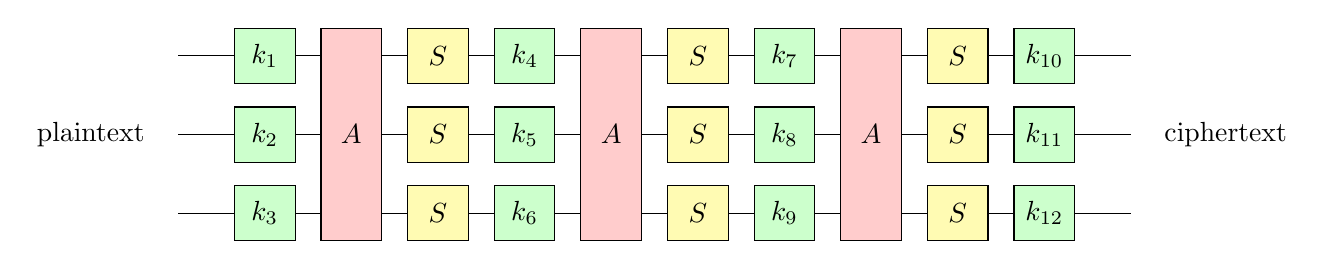
\begin{tikzpicture}[xscale=1.1,
      a/.style={fill=red!20},
      s/.style={fill=yellow!30},
      k/.style={fill=green!20}]
      \draw (0,2) -- (11,2);
      \draw (0,1) node[left=2ex]{plaintext} -- (11,1) node[right=2ex]{ciphertext};
      \draw (0,0) -- (11,0);
      \draw[k] (1,2) +(-0.35,-0.35) rectangle node{$k_1$} +(0.35,0.35);
      \draw[k] (1,1) +(-0.35,-0.35) rectangle node{$k_2$} +(0.35,0.35);
      \draw[k] (1,0) +(-0.35,-0.35) rectangle node{$k_3$} +(0.35,0.35);
      \draw[a] (2,0) +(-0.35,-0.35) rectangle node{$A$} +(0.35,2.35);
      \draw[s] (3,2) +(-0.35,-0.35) rectangle node{$S$} +(0.35,0.35);
      \draw[s] (3,1) +(-0.35,-0.35) rectangle node{$S$} +(0.35,0.35);
      \draw[s] (3,0) +(-0.35,-0.35) rectangle node{$S$} +(0.35,0.35);
      \draw[k] (4,2) +(-0.35,-0.35) rectangle node{$k_4$} +(0.35,0.35);
      \draw[k] (4,1) +(-0.35,-0.35) rectangle node{$k_5$} +(0.35,0.35);
      \draw[k] (4,0) +(-0.35,-0.35) rectangle node{$k_6$} +(0.35,0.35);
      \draw[a] (5,0) +(-0.35,-0.35) rectangle node{$A$} +(0.35,2.35);
      \draw[s] (6,2) +(-0.35,-0.35) rectangle node{$S$} +(0.35,0.35);
      \draw[s] (6,1) +(-0.35,-0.35) rectangle node{$S$} +(0.35,0.35);
      \draw[s] (6,0) +(-0.35,-0.35) rectangle node{$S$} +(0.35,0.35);
      \draw[k] (7,2) +(-0.35,-0.35) rectangle node{$k_7$} +(0.35,0.35);
      \draw[k] (7,1) +(-0.35,-0.35) rectangle node{$k_8$} +(0.35,0.35);
      \draw[k] (7,0) +(-0.35,-0.35) rectangle node{$k_9$} +(0.35,0.35);
      \draw[a] (8,0) +(-0.35,-0.35) rectangle node{$A$} +(0.35,2.35);
      \draw[s] (9,2) +(-0.35,-0.35) rectangle node{$S$} +(0.35,0.35);
      \draw[s] (9,1) +(-0.35,-0.35) rectangle node{$S$} +(0.35,0.35);
      \draw[s] (9,0) +(-0.35,-0.35) rectangle node{$S$} +(0.35,0.35);
      \draw[k] (10,2) +(-0.35,-0.35) rectangle node{$k_{10}$} +(0.35,0.35);
      \draw[k] (10,1) +(-0.35,-0.35) rectangle node{$k_{11}$} +(0.35,0.35);
      \draw[k] (10,0) +(-0.35,-0.35) rectangle node{$k_{12}$} +(0.35,0.35);
  \end{tikzpicture}
\end{equation*}
\end{definition}

Note that the three basic steps (key mixing, diffusion, and S-box
application) are repeated several times; each such repetition is
called a \textbf{round}%
\index{cipher!round}%
\index{rounds of a cipher} of the block cipher.  The more rounds a
block cipher has, the better its diffusion and non-linearity
properties. The final round is short: it only consists of a key
mixing step, with no final diffusion or S-box application. The reason
is that performing a final diffusion and S-box application would not
add anything to the security of the cipher. An attacker could simply
undo these last two steps, since they do not depend on the key.

The matrix $A$ is called the \textbf{diffusion matrix}%
\index{diffusion matrix}%
\index{matrix!diffusion}%
\index{cipher!diffusion matrix} of the cipher. Note that, unlike for
the Hill cipher, the matrix $A$ is fixed once and for all and is not
part of the key. Instead, the key consists of scalars that are added
to the current block at the beginning of each round.

\begin{example}{Toy block cipher: encryption}{toy-block-cipher-encryption}
  Encrypt the message ``I like math'' using the block cipher of
  Definition~\ref{def:toy-block-cipher} and the key
  $1,1,3,3,5,5,7,7,9,9,11,11$.
\end{example}

\begin{solution}
  We first represent the plaintext as a sequence of blocks, padding
  the final block with zeros:
  \begin{equation*}
    \mbox{Plaintext blocks:}\quad
    (9,0,12),\
    (9,11,5),\
    (0,13,1),\
    (20,8,0).
  \end{equation*}
  To encrypt the first block, we start with the vector
  $\mat{9,0,12}^T$ and apply the following steps:

  \noindent{\bf Round 1:}
  \begin{itemize}
  \item Key mixing: the first three components of the key are
    $1,1,3$. We add them to the plaintext.
    \begin{equation*}
      \begin{mymatrix}{c} 9 \\ 0 \\ 12 \end{mymatrix}
      +
      \begin{mymatrix}{c} 1 \\ 1 \\ 3 \end{mymatrix}
      ~=~
      \begin{mymatrix}{c} 10 \\ 1 \\ 15 \end{mymatrix}.
    \end{equation*}
  \item Diffusion: multiply by the matrix $A$.
    \begin{equation*}
      \begin{mymatrix}{ccc}
        1 & 2 & 3 \\
        3 & 1 & 2 \\
        2 & 3 & 1 \\
      \end{mymatrix}
      \begin{mymatrix}{c} 10 \\ 1 \\ 15 \end{mymatrix}
      ~=~
      \begin{mymatrix}{c} 28 \\ 3 \\ 9 \end{mymatrix}.
    \end{equation*}
  \item S-box application: apply the S-box to each component of the
    vector.
    \begin{equation*}
      \begin{mymatrix}{c} S(28) \\ S(3) \\ S(9) \end{mymatrix}
      ~=~
      \begin{mymatrix}{c} 8 \\ 2 \\ 18 \end{mymatrix}.
    \end{equation*}
  \end{itemize}

  \noindent{\bf Round 2:}
  \begin{itemize}
  \item Key mixing: the next three components of the key are
    $3,5,5$.
    \begin{equation*}
      \begin{mymatrix}{c} 8 \\ 2 \\ 18 \end{mymatrix}
      +
      \begin{mymatrix}{c} 3 \\ 5 \\ 5 \end{mymatrix}
      ~=~
      \begin{mymatrix}{c} 11 \\ 7 \\ 23 \end{mymatrix}.
    \end{equation*}
  \item Diffusion:
    \begin{equation*}
      \begin{mymatrix}{ccc}
        1 & 2 & 3 \\
        3 & 1 & 2 \\
        2 & 3 & 1 \\
      \end{mymatrix}
      \begin{mymatrix}{c} 11 \\ 7 \\ 23 \end{mymatrix}
      ~=~
      \begin{mymatrix}{c} 7 \\ 28 \\ 8 \end{mymatrix}.
    \end{equation*}
  \item S-box application:
    \begin{equation*}
      \begin{mymatrix}{c} S(7) \\ S(28) \\ S(8) \end{mymatrix}
      ~=~
      \begin{mymatrix}{c} 26 \\ 8 \\ 16 \end{mymatrix}.
    \end{equation*}
  \end{itemize}

  \noindent{\bf Round 3:}
  \begin{itemize}
  \item Key mixing: the next three components of the key are
    $7,7,9$.
    \begin{equation*}
      \begin{mymatrix}{c} 26 \\ 8 \\ 16 \end{mymatrix}
      +
      \begin{mymatrix}{c} 7 \\ 7 \\ 9 \end{mymatrix}
      ~=~
      \begin{mymatrix}{c} 4 \\ 15 \\ 25 \end{mymatrix}.
    \end{equation*}
  \item Diffusion:
    \begin{equation*}
      \begin{mymatrix}{ccc}
        1 & 2 & 3 \\
        3 & 1 & 2 \\
        2 & 3 & 1 \\
      \end{mymatrix}
      \begin{mymatrix}{c} 4 \\ 15 \\ 25 \end{mymatrix}
      ~=~
      \begin{mymatrix}{c} 22 \\ 19 \\ 20 \end{mymatrix}.
    \end{equation*}
  \item S-box application:
    \begin{equation*}
      \begin{mymatrix}{c} S(22) \\ S(19) \\ S(20) \end{mymatrix}
      ~=~
      \begin{mymatrix}{c} 6 \\ 15 \\ 10 \end{mymatrix}.
    \end{equation*}
  \end{itemize}

  \noindent{\bf Round 4 (the final round is abbreviated):}
  \begin{itemize}
  \item Key mixing: the next three components of the key are
    $9,11,11$.
    \begin{equation*}
      \begin{mymatrix}{c} 6 \\ 15 \\ 10 \end{mymatrix}
      +
      \begin{mymatrix}{c} 9 \\ 11 \\ 11 \end{mymatrix}
      ~=~
      \begin{mymatrix}{c} 15 \\ 26 \\ 21 \end{mymatrix}.
    \end{equation*}
  \end{itemize}
  Therefore, the first ciphertext block is $(15,26,21)$. We repeat the
  same procedure with the remaining plaintext blocks, and obtain the
  following ciphertext blocks:
  \begin{equation*}
    \mbox{Ciphertext blocks:}\quad
    (15,26,21),\
    (7,24,1),\
    (2,16,23),\
    (7,20,22).
  \end{equation*}
  The corresponding ciphertext is $\q{OZUGXABPWGTV}$.
\end{solution}

Are ciphers like this actually used in the real world? The answer
is yes. While the cipher of Definition~\ref{def:toy-block-cipher} is
greatly simplified, it has the same basic structure as modern
real-world block ciphers (such as AES, the Advanced Encryption
Standard). Naturally, these real-world ciphers differ in some details,
such as the alphabet size, the block size, the number of rounds, the
design of the S-boxes, the way the key is computed, and the precise
order in which the operations are applied. However, their basic
structure is very similar to our toy cipher, and indeed, all such
ciphers rely on key mixing, diffusion, and non-linear S-boxes as
their key components.

For example, AES uses an alphabet size of $256$ instead of $29$ (i.e.,
it operates on bytes%
\index{byte}, rather than elements of $\Z_{29}$). Although $\Z_{256}$
is not a field (because $256$ is not prime), it nevertheless turns out
that there exists a field with $256$ elements, and AES uses it for its
algebraic operations. Our toy cipher's block size of $3$ is much too
small to achieve effective diffusion; modern real-world ciphers use
block sizes between $16$ and $32$ bytes ($128$ to $256$ bits). The
design of the S-boxes is a bit of a black art; at minimum, they must
be designed to withstand two common types of cryptanalysis known as
\textbf{linear cryptanalysis}%
\index{cryptanalysis!linear}%
\index{linear cryptanalysis} and \textbf{differential cryptanalysis}%
\index{cryptanalysis!differential}%
\index{differential cryptanalysis}.  Among other things, this means
that the S-box should be ``as far from linear'' as possible.

A detailed discussion of the design and cryptanalysis of modern block
ciphers is far beyond the scope of this book, but we hope that you
have gotten a taste of this fascinating subject, and the role that
linear algebra over finite fields plays in it.
